\section{TensorFlow Lite no ESP32}

Primeiramente foi realizado uma validação simples da implementação de uma rede neural no ESP32 utilizando a  biblioteca TensorFlow Lite.

Para isso foi validado um exemplo de aplicação encontrado no github onde o autor utilizou a biblioteca em conjunto com
a plataforma de desenvolvimento PlatformIO para a classificar se entre duas variáveis float aleatórias de input o segundo valor é maior.
Essa simples aplicação tem sua acurácia facilmente verificada pois basta uma operação de comparação.

Quanto ao funcionamento da biblioteca, a rede neural a ser utilizado é modelada e treinada na plataforma do TensorFlow e um arquivo 
de configuração hexadecimal é gerado. Esse arquivo é adicionado ao firmware e interpretado pela biblioteca TensorFlow Lite de forma 
a implementar essa rede e gerar as inferências desejadas.

Na Figura 1 vemos o resultado do teste implementado disponível na saída serial do microcontrolador. Nele vemos os dois valores aleatórios
de input seguidos do resultado da inferência e o resultado esperado.

\begin{figure}[h!]
    \centering
    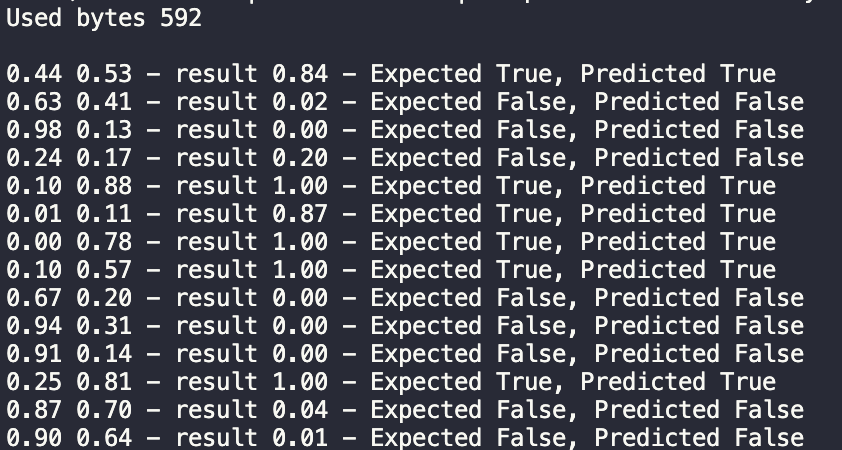
\includegraphics[scale=0.5]{images/resultTESTE.png}
    \caption{Resultados do teste realizado.}
\end{figure}
